\documentclass{article}

\usepackage{lipsum}  % add tests \lipsum
\usepackage{tikz}
\usepackage{amsmath}  % math
\usepackage{graphics} % images
\usepackage{hyperref} % links
\usepackage[          
    top=2cm,
    bottom=2cm,
    left=3cm,
    right=3cm
]{geometry}           % margins
\usepackage{pgfplots} % simplify graphs
\usepackage{float}    % add directive on figures
\usepackage{placeins} % Add \FloatBarrier for figures
%\usepackage[section]{placeins} % or here, automatically insert a \FloatBarrier at the end of every sections
\usepackage{setspace} % better lines spacing (inside paragraphs) (more breathing space), triggered with \onehalfspacing... 
\usepackage{parskip}  % removes paragraph indentation + add clean separation between paragrapgh, but we can 
                      % still control vertical space manually withh \setlength{\parskip}{1em}...
\usepackage[T1]{fontenc} % use T1 font encoding -> accented character...
\usepackage{lmodern}     % Latin Modern font, supports well T1 encoding
\usepackage{microtype}   % better micro spacing (letters/words)
\usepackage{fancyhdr}    % page headers
\usepackage{titlesec}    % used for sections style here, \titleformat
\usepackage{xcolor}      % coors text with \textcolor
\usepackage{tcolorbox}   % used to highlight text, literaly a colored box
\usepackage{listings}    % used for code-blocks
\usepackage{minted}      % used for code-blocks (alterntive) - more powerfull but rely on python - require `pdflatex -shell-escape file.tex`
\usepackage{multicol}    % handle multicolumns cleanly 
\usepackage{pgf-pie}     % pie-chart
\usepackage{xstring}     % beter for string programming
\usepackage{chemfig}     % for drawing molecules
\usepackage{pgfplotstable} %read csv 

% for \path[name intersections={of=f and g}];
\usetikzlibrary{intersections} 
\usetikzlibrary{trees} % you know its use just by its name lol
\usetikzlibrary{3d} % enables 3d coordinates system
\usetikzlibrary{shapes.geometric}

%%%%%%% hyperref %%%%%%%
\hypersetup{colorlinks = true,
            linkcolor=blue,
            urlcolor=blue
}
%%%%%%%%%%%%%%%%%%%%%%%%%

%%%%%%% fancyhdr %%%%%%%

\fancyhf{}
\pagestyle{fancy}

%%% page headers %%%
\fancyhead[L]{Doc}
\fancyhead[R]{J LP}
\fancyfoot[C]{\thepage}
\setlength{\headheight}{15pt}
%%%%%%%%%%%%%%%%%%%%
%%%%%%%%%%%%%%%%%%%%%%%%%

%%%%%%%%%% titlesec %%%%%%%%%
\titleformat{\section}{\large\bfseries}{\thesection}{1em}{}
%%%%%%%%%%%%%%%%%%%%%%%%%


%%%%%% listings configurations %%%%

%\lstset{ % define globally, but risks of flickering
%    basicstyle=\ttfamily\small,
%    keywordstyle=\color{blue},
%    commentstyle=\color{red!70!black},
%    stringstyle=\color{green!50!black},
%    breaklines=true,
%    keepspaces=true,
%    showstringspaces=false,
%    backgroundcolor=\color{gray!50},
%    frame=single
%}

% or define a style variable

\tcbuselibrary{listings}

% no flickering
\newtcblisting{codebox1}{
    listing only,
    colback=gray!5,
    colframe=gray!30,
    arc=4pt,
    boxrule=0.5pt,
    listing options={
        language=C++,
        basicstyle=\ttfamily\small,
        keywordstyle=\color{blue},
        commentstyle=\color{gray},
        stringstyle=\color{green!50!black},
        breaklines=true,
        keepspaces=true,
        columns=fullflexible,
        showstringspaces=false
    }
}

%%%%%%%%%%%%%%%%%%%%%%%%%%%%%%%

%%%%%%% minted %%%%%%

\usemintedstyle{friendly}
% friendly
% colorful
% murphy
% native
% monokai

%%%%%%%%%%%%%%%%%%%%%%%%%%%%%%%

%%%%%%% Multi-Column spacing %%%%%%%

\setlength{\columnsep}{1cm}

%%%%%%%%%%%%%%%%%%%%%%%%%%%%%%%

%%%%%%% Footnote spacing %%%%%%%

\setlength{\skip\footins}{2em}

%%%%%%%%%%%%%%%%%%%%%%%%%%%%%%%

\usepgfplotslibrary{fillbetween}
\usepgfplotslibrary{statistics}
% \usepgfplotslibrary{colormaps} %cool theme colormap/themename

\pgfplotsset{compat=1.18}

\pgfplotsset{ %define custom pgfplot theme, heatmap
  colormap={inferno}{
    rgb255(0cm)=(0,0,4);
    rgb255(1cm)=(31,12,72);
    rgb255(2cm)=(85,15,109);
    rgb255(3cm)=(136,34,106);
    rgb255(4cm)=(186,54,85);
    rgb255(5cm)=(227,89,51);
    rgb255(6cm)=(249,140,10);
    rgb255(7cm)=(249,201,50);
    rgb255(8cm)=(252,255,164);
  }
}

\title{Doc}
\author{J LP}
\date{\today}

%%%% VARIABLES REGISTRATION %%%

\newcommand{\mybloglink}{https://julienlargetpiet.tech}
\newcommand{\mybloglinkraw}{\url{https://julienlargetpiet.tech}}

\definecolor{mycolor1}{HTML}{1E90FF}
\definecolor{linkcolor1}{HTML}{4F9AD6}

%%%%%%%%%%%%%%%%%%%%%%%%%%%%%%%

%%%% FUNCTIONS REGISTRATION %%%

\newcommand{\link}[2]{\href{#1}{#2}}

%%%%%%%%%%%%%%%%%%%%%%%%%%%%%%%

\includeonly{ici}

\begin{document}

\onehalfspacing
\maketitle
{ % here we just do a scoping to define temporary hyperefsetup just used by \tableofcontents
  \hypersetup{linkcolor = black} 
  \tableofcontents
}

%%%%%% THIS IS EXTREMELY COOL LOOK AT THAT %%%%%%%
% 
%\pgfplotstableread[col sep=comma]{pie.csv}\datatable
%
%\def\result{}%
%\pgfplotstablegetrowsof{\datatable}
%\pgfmathtruncatemacro{\nrows}{\pgfplotsretval-1}
%
%\foreach \i in {0,...,\nrows} {
%    \pgfplotstablegetelem{\i}{value}\of{\datatable}
%    \let\val\pgfplotsretval
%    \pgfplotstablegetelem{\i}{label}\of{\datatable}
%    \let\lab\pgfplotsretval
%
%    \ifx\result\empty
%        \xdef\result{\val/{\text{\lab}}}
%    \else
%        \xdef\result{\result,\val/{\text{\lab}}}
%    \fi
%}
%
%%%%%%%%%%%%%%%%%%%%%%%%%%%%%


\section{Raw text}

\lipsum

\section{Basics - sections, subsections, paragraphs...}
\subsection{Normal}

Hello Normal

\subsubsection{Normal}

A paragraph yeah a paragraph haha, lol i dk what to write here so i rpetend just to write sentences that make sens whil it is pure nonsens. 

\subsubsection{Normal2}

Comon we do it again
A paragraph yeah a paragraph haha, lol i dk what to write here so i rpetend just to write sentences that make sens whil it is pure nonsens. 

\paragraph{Important paragraph}

A paragraph yeah a paragraph haha, lol i dk what to write here so i rpetend just to write sentences that make sens whil it is pure nonsens. 
Comon we do it again
A paragraph yeah a paragraph haha, lol i dk what to write here so i rpetend just to write sentences that make sens whil it is pure nonsens. 

\subparagraph{Important sub-paragraph}

A sub-paragraph yeah a sub-paragraph haha, lol i dk what to write here so i rpetend just to write sentences that make sens whil it is pure nonsens. 
Comon we do it again
A paragraph yeah a paragraph haha, lol i dk what to write here so i rpetend just to write sentences that make sens whil it is pure nonsens. 

\textbf{Hello in bold} 

\textit{Hello in italic} 

\underline{Hello underlined} 

\underline{\textbf{\textit{Hello all}}} 

\section{Font Sizes}

{\tiny tiny}

{\footnotesize footnotesize}

{\small small}

{\normalsize normalsize}

{\large large}

{\Large Large}

{\huge huge}

{\Huge Huge}

\section{Footnotes}

Hell0\footnote{this is a first footnote}

Hell02\footnote{this is a second footnote}

\section{Special characters you must escape with \textbackslash}

\$

\%

\$

\_

\section{Links}

\href{\mybloglink}{My-blog}

%% OR directly show url
\url{\mybloglink}

% with variable call

\mybloglinkraw

% with function call

\link{\mybloglink}{My-blog}

\section{Xcolors}

\textcolor{blue}{Important}

\textcolor{mycolor1}{Important} % call to mycolor1 defined in preamble with \definecolor

\textcolor[HTML]{FF5733}{Important} % inline call of HTML colors (hexadecimal)


\section{Highligts}

Default coloredbox

\begin{tcolorbox}
This is a highlighted block
\end{tcolorbox}

Customoized tcolorbox

\begin{tcolorbox}[
    colback=blue!10,
    colframe=blue!5!green
]
This is a second highlighted block
\end{tcolorbox}

Customoized 2 tcolorbox

\begin{tcolorbox}[
    colback=blue!10,
    colframe=mycolor1
]
This is a second highlighted block
\end{tcolorbox}

Customoized 3 tcolorbox

\begin{tcolorbox}[
    colback=gray!10,
    colframe=gray!50,
    coltitle=blue,
    colbacktitle=orange!5,
    arc=6pt,
    boxrule=0.5pt,
    title=Hell Yeah Title,
]
Clean modern box
\end{tcolorbox}

\section{Math}

Some Math:

\[
    \int_0^1 x^2 dx = \frac{1}{3}
\]

Inline maths:

$\int_0^1 x^2 dx = \frac{1}{3}$

\section{Code-Block}

First, with verbatim

\begin{verbatim}
int main() {
    return 0;
}
\end{verbatim}

Now with listings

%Global version settings:
%
%\begin{lstlisting}[language=C++]
%#include <iostream.h>
%
%int main() {
%    std::string x = "this is a string";
%    std::cout << x << "\n";
%    // comment
%    return 0;
%}
%\end{lstlisting}

Variable version settings:

\begin{codebox1}
#include <iostream.h>

int main() {
    std::string x = "this is a string";
    std::cout << x << "\n";
    // comment
    return 0;
}
\end{codebox1}

With minted (best imo):

\begin{tcolorbox}[colback=gray!5, colframe=gray!30, arc=4pt]
\begin{minted}{cpp}
#include <iostream.h>

int main() {
    std::string x = "this is a string";
    std::cout << x << "\n";
    // comment
    return 0;
}
\end{minted}
\end{tcolorbox}


\section{Lists}

\begin{itemize}
    \item First
    \item Second
\end{itemize}

Numbered Lists:

\begin{enumerate}
    \item First
    \item Second
\end{enumerate}

\section{Tables}

\begin{tabular}{|c|c|}
\hline
    A & B \\
\hline
    C & D \\
\hline
\end{tabular}

\section{Images}

%\begin{figure}[H]
%    \centering
%    
\includegraphics[width=0.5\textwidth]{cc2.png}
%    \caption{Example Image}
%\end{figure}
\begin{figure}[htbp]
    \centering
    
\includegraphics[width=0.5\textwidth]{cc2.png}
    \caption{Example Image}
\end{figure}
\FloatBarrier

\section{Expansions}

\subsection{Variables (Macro basiques)}

\def\a{Rémi}
\def\b{Julien}

% "\ " is to define a space, we need to do that because the macro eats the following space
Bonjour \a\ et \b.

Bonjour \a{} et \b.

\subsection{Macro - Extended}

\newcommand{\hello}[3]{Hello #1, #2 et #3}

\hello{Rémi}{Julien}{Lucas}

\subsection{Les conditions}

% we escape underscore
\ifnum 5 > 3
OUI\_1
\else
NO\_1
\fi

\ifx\a\b
OUI\_2
\else
NO\_2
\fi

\ifx\aRémi
OUI\_2B
\else
NO\_2B
\fi

\IfStrEq{\a}{Rémi}{YES}{NO}

\def\a{\b}

% output NO_3 because it is "literally" different ("\b" -> literally)
% in order to get the real value, we got to expand it, with \edef 
\ifx\a\b
OUI\_3
\else
NO\_3
\fi

\edef\a{\b}

\ifx\a\b
OUI\_4
\else
NO\_4
\fi

% compare la longueur
\ifdim 2cm>1cm
OUI\_5
\else
NO\_5
\fi

% \newif

\newif\ifcool
\cooltrue

\ifcool
OUI\_6
\else
NO\_6
\fi

\coolfalse

\ifcool
OUI\_6
\else
NO\_6
\fi

\iftrue
OUI\_7
\fi

% same pattern as following:

\def\coolb{\iftrue or \iffalse}
\def\coolbtrue{\let\coolb\iftrue}
\def\coolbfalse{\let\coolb\iffalse}

\coolbtrue

\coolb
OUI\_8
\else
NO\_8
\fi

\coolbfalse

\coolb
OUI\_9
\else
NO\_9
\fi

\subsection{Check Emptyness}

\def\x{}

\ifx\x\empty
EMPTY
\else
NOT EMPTY
\fi

\subsection{Loop}

\foreach \xb in {1,2,3,4} {
    \IfStrEq{\xb}{4}{END}{Value: \xb \\} 
}

\def\lst{1,2,3,4}

\foreach \xb in \lst {
    \IfStrEq{\xb}{4}{END}{Value: \xb \\} 
}

\def\lstb{}
\edef\lst{\lstb 1}
\edef\lst{\lstb,2}
\edef\lst{\lstb,2}
\edef\lst{\lstb,3}

\foreach \xb in \lstb {
    \IfStrEq{\xb}{4}{END}{Value: \xb \\} 
}

% PATTERN MATCHING

\def\pairs{{A/1},{B/2},{C/3},{D/4}}

\foreach \x/\y in \pairs {
    \x : \y \\
}

\def\pairsb{{A/1/A1},{B/2/B2},{C/3/C3},{D/4/D4}}

\foreach \x/\y/\z in \pairsb {
    \x : \y : \z \\
}


\def\pairsb{{A/{1/A1}},{B/{2/B2}},{C/{3/C3}},{D/{4/D4}}}

\def\splittemp#1/#2-{
    \x : #1 - #2 \\
}

\foreach \x/\temp in \pairsb {
    \expandafter\splittemp\temp-
}

% \relax does nothing, just a token to be consumed

\def\splittemp#1/#2\relax{
    \x : #1 - #2 \\
}

\foreach \x/\temp in \pairsb {
    \expandafter\splittemp\temp\relax
}

\subsection{Expandre un arbre}

\def\pairsc{{N1/{L/V1}},{N2/{R/V2}},{N3/{{L/V3}/{R/V4}}},{N4/{{L/{{L/V5}/{R/V6}}}/{R/V7}}}}

\newcommand{\treeleaf}[1]{%
    \IfStrEq{#1}{L}
        {Side: #1}
        {%
            \IfStrEq{#1}{R}
                {Side: #1}
                {Value: #1}%
        }%
}

\newcommand{\treesplit}[1]{%
    \IfSubStr{#1}{/}
        {%
            \expandafter\treesplitaux#1\relax
        }
        {%
            \treeleaf{#1}%
        }%
}

\def\treesplitaux#1/#2\relax{%
    (%
    \treesplit{#1}%
    /%
    \treesplit{#2}%
    )%
}

\foreach \x/\temp in \pairsc {%
    \x : \expandafter\treesplit\temp \\
}

% \expandafter A B
% 
% means:
% 
% expand B FIRST, then apply A

\newpage

\subsection{Tikz - Trees}

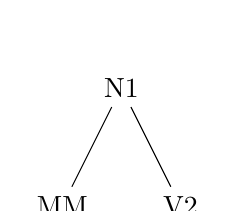
\begin{tikzpicture}

    \node{N1} child{ node{MM} } child{ node{V2} };

\end{tikzpicture}

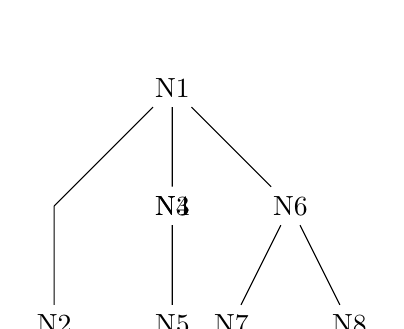
\begin{tikzpicture}

    \node{N1} 
        child{ child{node{N2}}  } 
        child{ 
            node{N3} 
            node{N4}
                child { 
                      node{N5} 
                  } 
            }
        child {
            node{N6} child {node{N7}} child {node{N8}}
        };

\end{tikzpicture}


\subsubsection{L'arbre prend forme}

En fait j'ai pas réusii, il vaut mieux générer la structure statique avec python, R ou autre puis le mettre dans un include/input.

%\newlength{\A}
%\newlength{\B}
%\setlength{\A}{0.5\textwidth}
   
\newcommand{\treetikz}[1]{%
    \IfSubStr{#1}{/}
        {{\expandafter\treetikzsplit#1\relax}}
        {node {\treeleaf{#1}}}
}

\def\treetikzsplit#1/#2\relax{%
    node{N} child { \treetikz{#1} } child { \treetikz{#2} }
}

 
\newcommand{\treetikzB}[1]{%
    \IfSubStr{#1}{(}
        {\expandafter\treetikzsplitB#1\relax}
        {node {\treeleaf{#1}}}
}

\def\treetikzsplitB(#1,#2)\relax{%
    node {N}
      child { \treetikzB{#1} }
      child { \treetikzB{#2} }
}

%\foreach \x/\temp in \pairsc {%
%    \begin{tikzpicture}[
%      level distance=1.5cm,
%      sibling distance=2.5cm
%    ]
%
%        \node{\x} child {\treetikz{\temp}};
%    
%    \end{tikzpicture}
%    
%    \vspace{1cm}
%}

%\begin{tikzpicture}[
%  level distance=1.5cm,
%  sibling distance=2.5cm
%]
%
%    \node{N} child { \treetikzB{((L,V3),(R,V4))} };
%
%\end{tikzpicture}

\newpage

\section{Cool macro}

\def\lstc{1,2,3,4}

\newcommand{\isin}[4]{%
    \IfSubStr{,#2,}{,#1,}{#3}{#4}%
}

\isin{L}{L,R,TT}{OUI}{NON}

\section{Boxes}

\fbox{\makebox[5cm][l]{Hello}}
\fbox{\makebox[5cm][c]{Hello}}
\fbox{\makebox[5cm][r]{Hello}}

\newpage

\section{Includes, yess like C}

\subsection{Input - no newpage}

\input{ici.tex}

Je suis inclu - 2


\subsection{Real incudes}

\include{ici.tex}
Je suis inclu - 2


\section{Tikz}

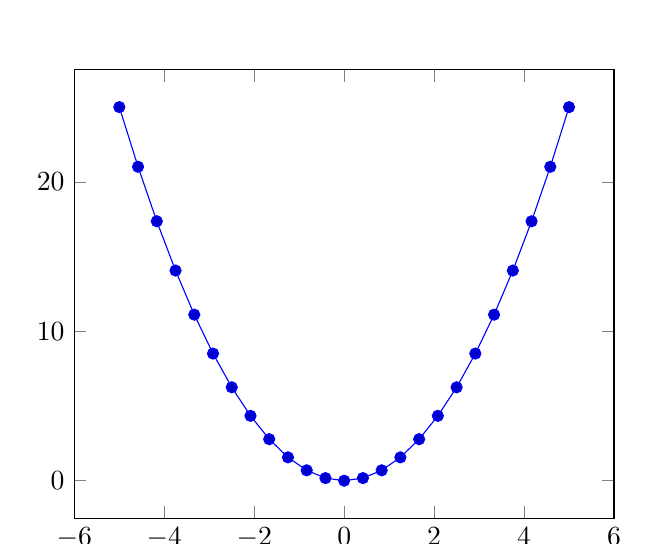
\begin{tikzpicture}
\begin{axis}

    \addplot{x^2};

\end{axis}
\end{tikzpicture}

\newpage
\section{MultiColumn - Nice for just text}
\subsection{Manual column breaking}

\begin{multicols}{2}

    This is col 1.

    \lipsum[1]

    \columnbreak

    This is col 2.

    \lipsum[2]

\end{multicols}

\newpage
\subsection{Auto column breaking}

\begin{multicols}{2}

    \lipsum[1-3]

\end{multicols}

\newpage

\subsection{Minipage - You can use Tikz here for each column}

% Each block should take 48% of the page width
% figure and table can not go inside minipage

\noindent
\begin{minipage}{0.48\textwidth}

\lipsum[1]

\end{minipage}
\hfill
\begin{minipage}{0.48\textwidth}

    \centering
    
\includegraphics[width=0.35\textwidth]{cc2.png}

    %\vspace{1cm}
    \bigskip

    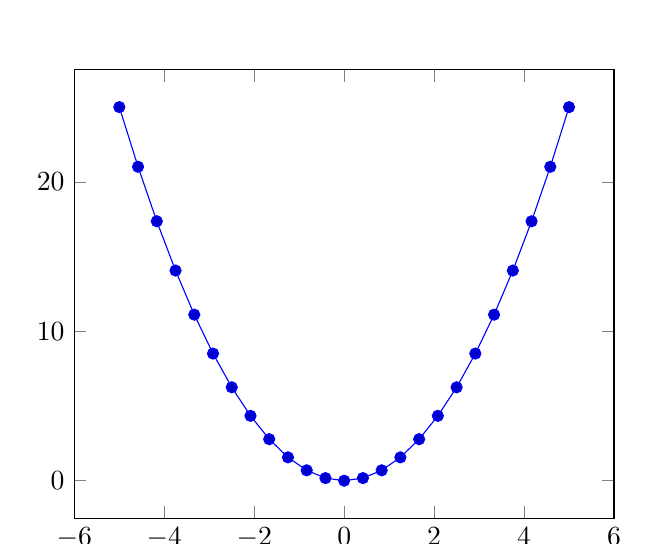
\begin{tikzpicture}
    \begin{axis}
    
        \addplot{x^2};
    
    \end{axis}
    \end{tikzpicture}

\end{minipage}

\newpage

\section{More on Tikz - pgfplots}
\subsection{2D graphs}

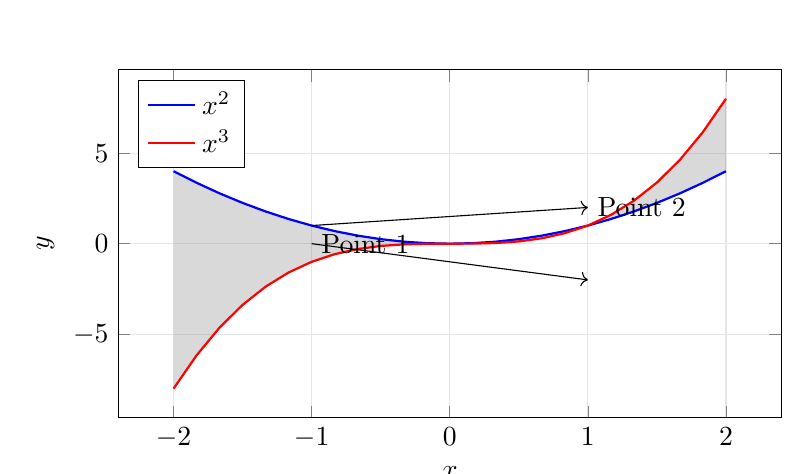
\begin{tikzpicture}
\begin{axis}[xlabel=$x$,
             ylabel=$y$,
             domain=-2:2,
             grid=both,
             grid style=gray!20,
             legend pos=north west,
             width=10cm,
             height=6cm]

    \addplot[name path = f,
             color=blue,
             thick]{x^2};

    \addplot[name path = g,
             color=red,
             thick]{x^3};

    \draw[->] (axis cs:-1,1) -- (axis cs:1,2) node[right] {Point 2};
    \draw[->] (axis cs:-1,0) node[right] {Point 1} -- (axis cs:1,-2);

    \addplot[gray,
             fill opacity = 0.3
    ] fill between [
        of = f and g
    ];

    % the order of legend correspond to the order of the \addplot 
    \addlegendentry{$x^2$}
    \addlegendentry{$x^3$}

\end{axis}
\end{tikzpicture}

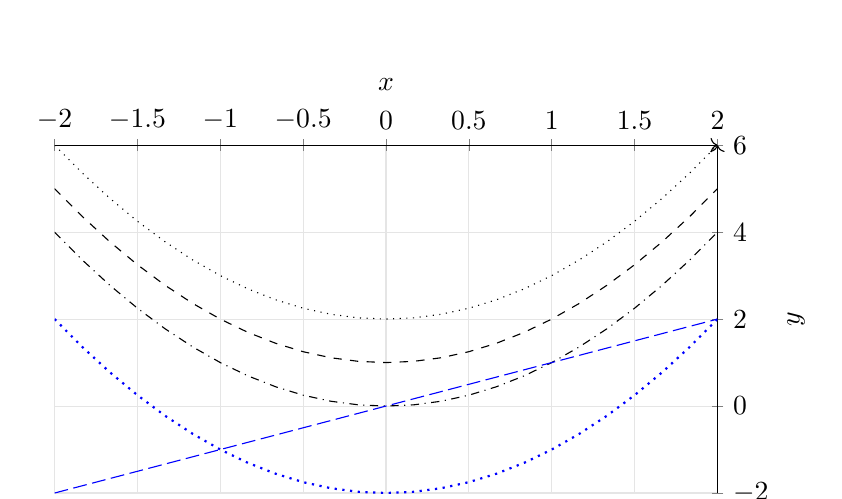
\begin{tikzpicture}
\begin{axis}[xlabel=$x$,
             ylabel=$y$,
             domain=-2:2,
             grid=both,
             axis lines=right,
             axis line style={->},
             grid style=gray!20,
             legend pos=north west,
             width=10cm,
             height=6cm]

% axis ine options:
% left
% right
% middle
% center
% box
% none

    \addplot[name path = f,
             color=blue,
             thick,
             dotted]{x^2 - 2};

    \addplot[dashed]{1 + x^2};
    \addplot[dotted]{2 + x^2};
    \addplot[dashdotted]{x^2};

% Custom dash

    \addplot[
        dash pattern=on 5pt off 2pt,
        color=blue
    ]{x^1};

\end{axis}
\end{tikzpicture}

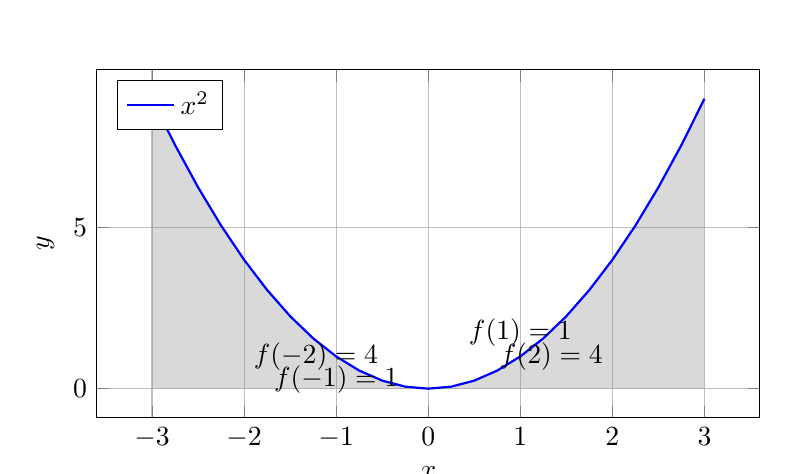
\begin{tikzpicture}
\begin{axis}[xlabel=$x$,
             ylabel=$y$,
             domain=-3:3,
             grid=both,
             legend pos=north west,
             width=10cm,
             height=6cm]

    \addplot[name path = f,
             color=blue,
             thick]{x^2};

    \node at (axis cs:1,1) [above] {$f(1)=1$};
    \node at (axis cs:-1,1) [below] {$f(-1)=1$};

    \node at (axis cs:2,1) [left] {$f(2)=4$};
    \node at (axis cs:-2,1) [right] {$f(-2)=4$};

    \addplot[name path = g,
             draw=none]{0*x};

    \addplot[gray,
             fill opacity = 0.3
    ] fill between [
        of = f and g
    ];

    \addlegendentry{$x^2$}

\end{axis}
\end{tikzpicture}

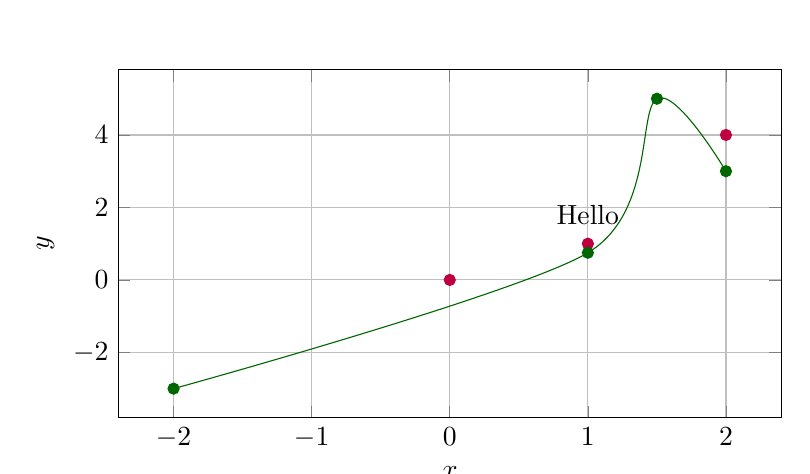
\begin{tikzpicture}
\begin{axis}[xlabel=$x$,
             ylabel=$y$,
             domain=-2:2,
             grid=both,
             legend pos=north west,
             width=10cm,
             height=6cm]

    \addplot[only marks,
             mark=*,
             color=purple] coordinates {
        (0, 0)
        (1, 1)
        (2, 4)
    };

    \addplot[mark=*,
             color=green!40!black,
             smooth] coordinates {
        (-2, -3)
        (1, 0.75)
        (1.5, 5)
        (2, 3)
    };

    \node at (axis cs:1,1.8) {Hello};

% ultra thin
% very thin
% thin
% semithick
% thick
% very thick
% ultra thick

\end{axis}
\end{tikzpicture}

\subsubsection{Scatterplot - CSV}

\begin{tikzpicture}
\begin{axis}[xlabel=$x$,
             ylabel=$y$,
             domain=-2:2,
             grid=both,
             legend pos=north west,
             width=10cm,
             height=6cm]

    \addplot[mark=*,
             only marks,
             color=red!40!black] table[col sep=comma,
                                       x=x,
                                       y=y] {scatterplot.csv};

\end{axis}
\end{tikzpicture}

\subsubsection{Scatterplot - CSV - Operations inside Table}

\begin{tikzpicture}
\begin{axis}[xlabel=$x$,
             ylabel=$y$,
             domain=-2:2,
             grid=both,
             legend pos=north west,
             width=10cm,
             height=6cm]

    \addplot[mark=*,
             only marks,
             color=red!40!black] table[col sep=comma,
                                       x=x,
                                       y expr=\thisrow{y} * 2 + \thisrow{y2}] {scatterplot.csv};

    \addplot[mark=*,
             only marks,
             color=blue!45] table[col sep=comma,
                                  x=x,
                                  y expr=\thisrow{y} * 2 * \thisrow{y2}] {scatterplot.csv};

    \addplot[mark=*,
             only marks,
             color=green!40] table[col sep=comma,
                                    x=x,
                                    y expr=\thisrow{y} * 2 + 2 * \thisrow{y2},
                                    restrict expr to domain={\thisrow{x}}{0:2}] {scatterplot.csv};
                            % `restrict expr to domain` expects two arguments:
                            %   1) an expression (here: \thisrow{x})
                            %   2) a domain interval (here: 0:2)
                            % Braces are required to delimit each argument explicitly,
                            % especially since \thisrow{x} is itself a macro with its own argument.
                            % So we write {\thisrow{x}}{0:2} to avoid ambiguity in TeX parsing.

\end{axis}
\end{tikzpicture}

\subsubsection{Scatterplot - CSV - Store in memory + Vertical concat}
 
\begin{tikzpicture}
\begin{axis}[xlabel=$x$,
             ylabel=$y$,
             domain=-2:8,
             grid=both,
             legend pos=north west,
             width=10cm,
             height=6cm]

    % global tables
    \pgfplotstableread[col sep=comma]{scatterplot.csv}\mytable

    \pgfplotstableread[col sep=comma]{scatterplot2.csv}\mytableB

    %concat mytableB to mytable
    \pgfplotstablevertcat{\mytable}{\mytableB}

    \pgfplotstablecreatecol[
        create col/expr={\thisrow{y}^2 - \thisrow{y2}}
    ]{y3}{\mytable}

    \addplot[mark=*,
             only marks,
             color=blue!45] table[col sep=comma,
                                  x=x,
                                  y expr=\thisrow{y3} * 2\thisrow{y2}] {\mytable};


\end{axis}
\end{tikzpicture}

\subsubsection{Intersections}

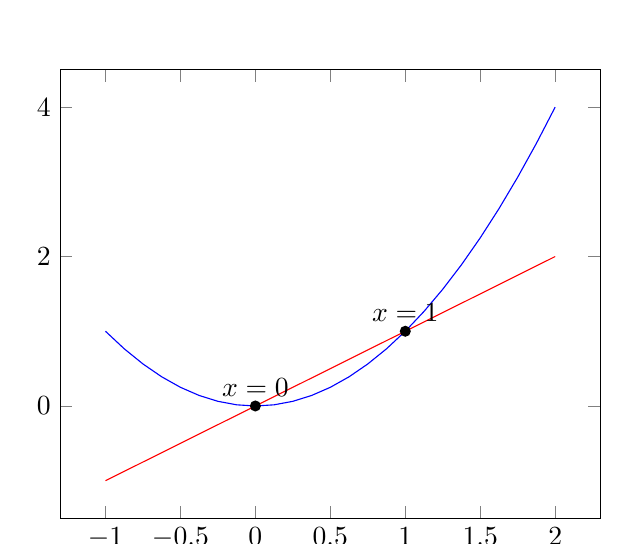
\begin{tikzpicture}
\begin{axis}[domain=-1:2]

    \addplot[name path=f, blue]{x^2};
    \addplot[name path=g, red]{x};
    
    % create the intersections "intersection-N"
    \path[name intersections={of=f and g}];
    
    \fill (intersection-1) circle (2pt);
    \fill (intersection-2) circle (2pt);

    \node at (intersection-1) [above] {$x=0$};
    \node at (intersection-2) [above] {$x=1$};

\end{axis}
\end{tikzpicture}

\subsection{Barplot}

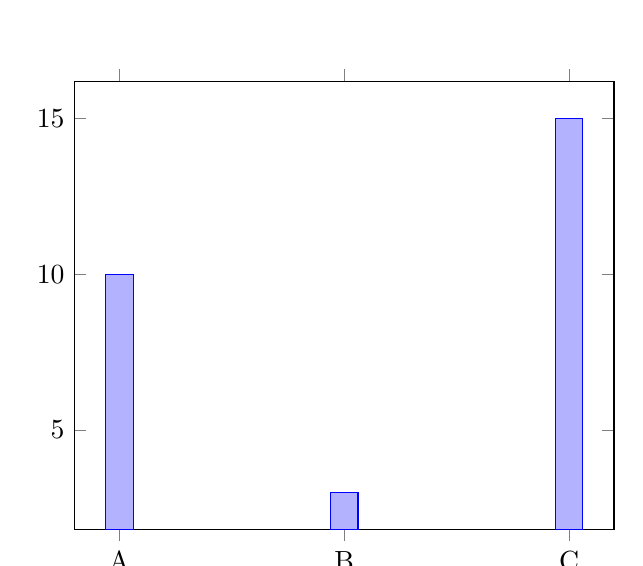
\begin{tikzpicture}
\begin{axis}[
    ybar,
    symbolic x coords={A,B,C},
    xtick=data
]

    \addplot coordinates {
        (A,10)
        (B,3)
        (C,15)
    };

\end{axis}
\end{tikzpicture}

\subsection{With CSV}

\begin{tikzpicture}
\begin{axis}[
    ybar,
    symbolic x coords={A,B,C},
    xtick=data
]

    \addplot[color=blue!50,
             fill=blue!50] table[col sep=comma,
                                 x=label,
                                 y=value] {barplot.csv};

\end{axis}
\end{tikzpicture}

\subsection{Rotating barplots}

\begin{tikzpicture}
\begin{axis}[
    xbar,
    symbolic y coords={A,B,C},
    ytick=data
]

    \addplot[color=blue!50,
             fill=blue!50] table[col sep=comma,
                                 y=label,
                                 x=value] {barplot.csv};

\end{axis}
\end{tikzpicture}

\subsubsection{Grouped Barplot}

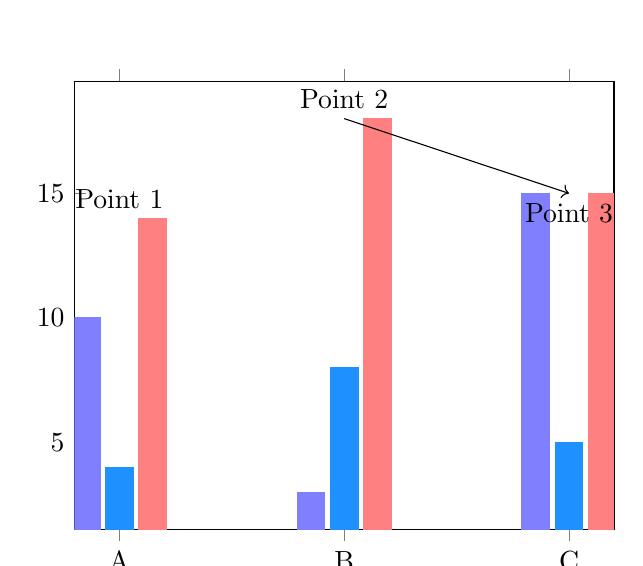
\begin{tikzpicture}
\begin{axis}[
    ybar,
    symbolic x coords={A,B,C},
    xtick=data
]

    \addplot[color=blue!50,
             fill=blue!50] coordinates {
        (A,10)
        (B,3)
        (C,15)
    };

    \addplot[color=mycolor1,
             fill=mycolor1] coordinates {
        (A,4)
        (B,8)
        (C,5)
    };

    \addplot[color=red!50,
             fill=red!50] coordinates {
        (A,14)
        (B,18)
        (C,15)
    };

    \node at (axis cs:A,14) [above] {Point 1};
    \node at (axis cs:B,18) [above] {Point 2};
    \draw[->] (axis cs:B,18) -- (axis cs:C,15) node[below] {Point 3};

\end{axis}
\end{tikzpicture}

\subsection{Histogramms + CSV}

\begin{tikzpicture}
\begin{axis}

    \addplot+[
        hist={bins=5, data min=1, data max=7, density},
        fill=blue!30,
        draw=black,
        mark=none
    ] table[col sep=comma,
            y=value] {histogramm.csv};

\end{axis}
\end{tikzpicture}

\subsection{Adding KDE plot}

\begin{tikzpicture} 
\begin{axis}

    \addplot+[
        hist={bins=5, data min=1, data max=7, density},
        fill=blue!30,
        draw=black,
        mark=none
    ] table[col sep=comma,
            y=value] {histogramm.csv};

    \addplot[
        smooth, thick, color=red
    ] table[
        col sep=comma, x=x, y=density
    ]{histogramm_kde.csv}; % never escapes "_" in filenames, only in text where we do "\_"

\end{axis}
\end{tikzpicture}

\subsection{Horizontal Boxplots + CSV}

\begin{tikzpicture}
\begin{axis}

    % +[...] keeps default, only add
    \addplot+[
        boxplot
    ] table[col sep=comma, 
            y=value] {boxplot.csv};

\end{axis}
\end{tikzpicture}

\subsection{Multiple histogramms + CSV}

\begin{tikzpicture}
\begin{axis}[
        ytick={1,2,3},
        yticklabels={A,B,C}
    ]

    \addplot+[
        boxplot,
        boxplot/draw position=1,
        fill=blue!20
    ] table[col sep=comma, 
            y=value] {boxplot.csv};

    \addplot+[
        boxplot,
        boxplot/draw position=2,
        fill=red!20
    ] table[col sep=comma, 
            y=value] {boxplot.csv};

    \addplot+[
        boxplot,
        boxplot/draw position=3,
        fill=orange!20
    ] table[col sep=comma, 
            y=value] {boxplot.csv};

\end{axis}
\end{tikzpicture}

\subsection{Vertical Boxplots + CSV}

\begin{tikzpicture}
\begin{axis}[
        xtick={1,2,3},
        xticklabels={A,B,C}
    ]

    \addplot+[
        boxplot,
        boxplot/draw direction=y,
        boxplot/draw position=1,
        fill=blue!20
    ] table[col sep=comma, 
            y=value] {boxplot.csv};

    \addplot+[
        boxplot,
        boxplot/draw direction=y,
        boxplot/draw position=2,
        fill=red!20
    ] table[col sep=comma, 
            y=value] {boxplot.csv};

    \addplot+[
        boxplot,
        boxplot/draw direction=y,
        boxplot/draw position=3,
        fill=orange!20
    ] table[col sep=comma, 
            y=value] {boxplot.csv};

\end{axis}
\end{tikzpicture}

\subsection{Pie Chart - Incomplete}

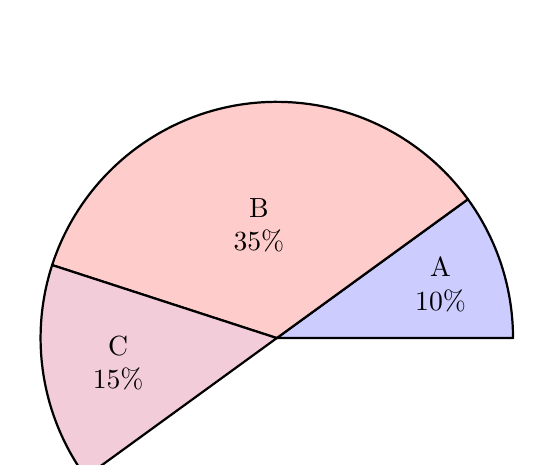
\begin{tikzpicture}
    \pie[
        color={blue!20, red!20,purple!20},
        text=inside
    ]{10/A, 35/B, 15/C}
\end{tikzpicture}

\subsubsection{Full Circle}

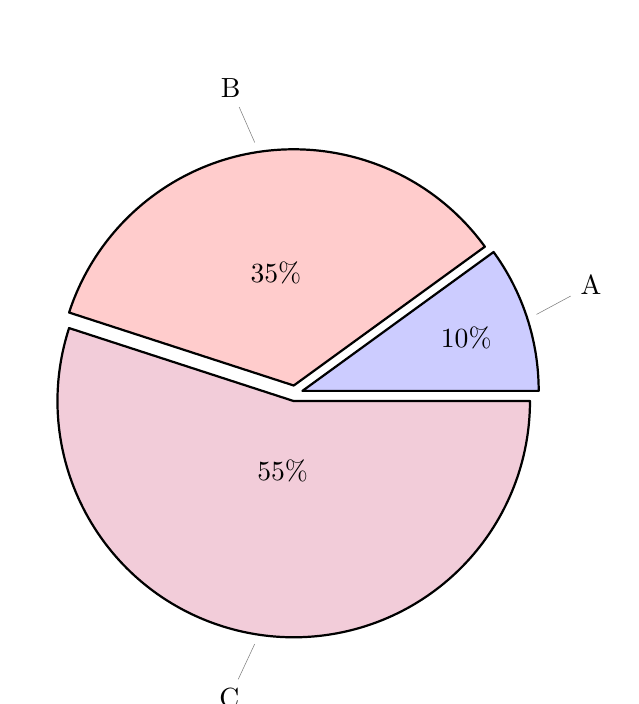
\begin{tikzpicture}
    \pie[
        color={blue!20, red!20,purple!20},
        text=pin,
        explode=0.1
    ]{10/A, 35/B, 55/C}
\end{tikzpicture}

\subsubsection{With CSV}

%\begin{tikzpicture}
%
%    \pie[
%        color={blue!20, red!20,purple!20},
%        text=pin,
%        explode=0.1
%    ]table[col sep=comma, label=label, value=value] {pie.csv}
%
%\end{tikzpicture}

\subsection{HeatMaps}

\subsubsection{Color interpolation}

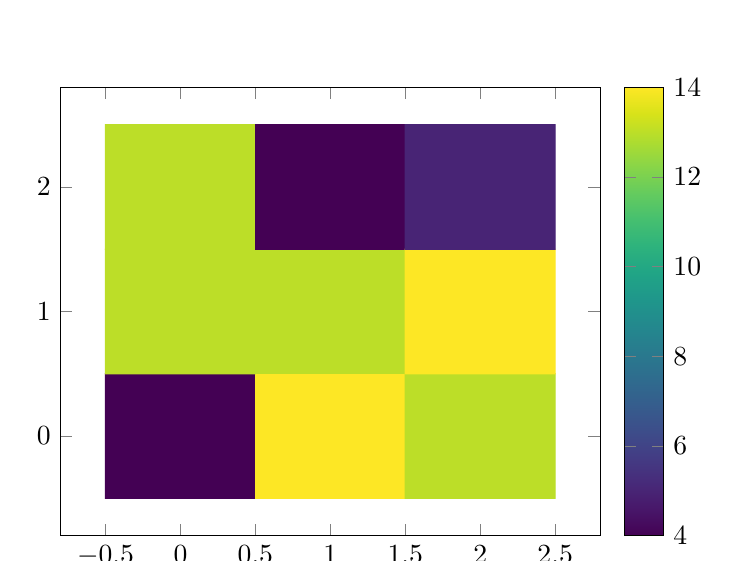
\begin{tikzpicture}
\begin{axis}[colorbar, 
             colormap name = viridis]

    % matrix plot* do color interpolation, it means that a cell colored is given
    % but still can get influenced by neighboors
    \addplot[matrix plot*,
             mesh/cols=3,
             point meta=explicit] coordinates {
        (0,0) [4] (1,0) [14] (2,0) [13]
        (0,1) [13] (1,1) [13] (2,1) [14]
        (0,2) [13] (1,2) [4] (2,2) [5]
    };

\end{axis}
\end{tikzpicture}

\section{3D graphs}

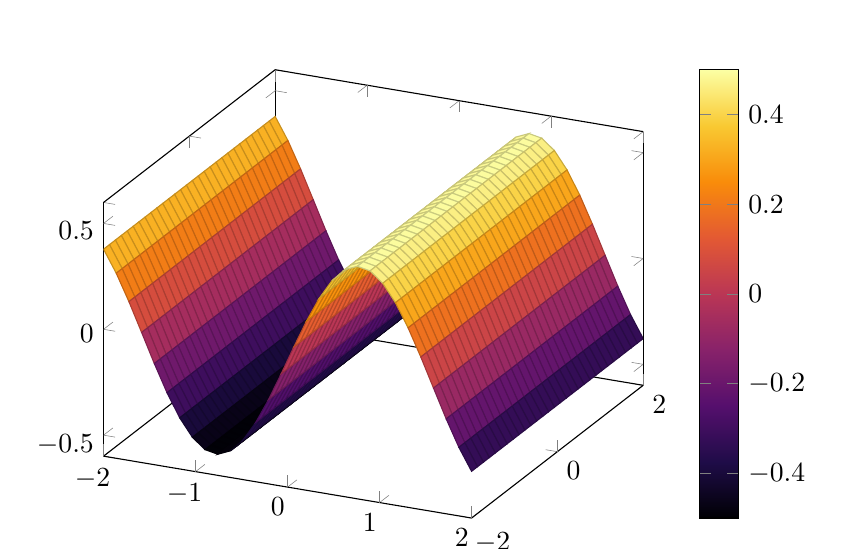
\begin{tikzpicture}
    \begin{axis}[colorbar,
                colormap name=inferno]

    \addplot3[surf,
              domain=-2:2, 
              y domain = -2:2,
              samples=30,
              samples y=30
    ]{sin(deg(x)) * cos(deg(x))};

\end{axis}
\end{tikzpicture}

\subsubsection{Fixed color}

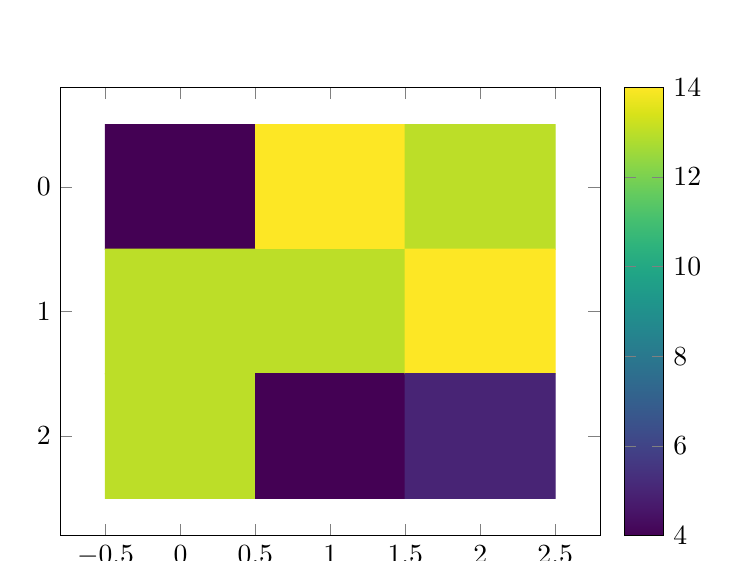
\begin{tikzpicture}
\begin{axis}[colorbar, 
             colormap name=viridis]

    \addplot[matrix plot,
             mesh/cols=3,
             point meta=explicit] coordinates {
        (0,0) [4] (1,0) [14] (2,0) [13]
        (0,1) [13] (1,1) [13] (2,1) [14]
        (0,2) [13] (1,2) [4] (2,2) [5]
    };

\end{axis}
\end{tikzpicture}

\subsubsection{CSV}
 
\begin{tikzpicture}
\begin{axis}[colorbar, 
             colormap name=inferno]

    \addplot[matrix plot,
             mesh/cols=3,
             point meta=explicit
    ] table[col sep=comma, 
            x=x,
            y=y,
            meta=value] {heatmap.csv};

\end{axis}
\end{tikzpicture}


\section{Tikz - Shapes}

\subsection{Triangle}

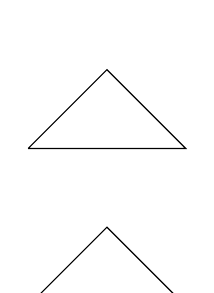
\begin{tikzpicture}

    \draw (0, 0) -- (1,1) -- (2,0) -- (0,0);

    %% or cycle back automatically
    \draw (0, -2) -- (1,-1) -- (2,-2) -- cycle;

\end{tikzpicture}

\subsection{Rectangle}

\begin{tikzpicture}

    \draw (0, 0) rectangle (3,2);

\end{tikzpicture}

\begin{tikzpicture}

    \draw (0, 0) -- (0,2) -- (3,2) -- (3,0) -- cycle;

\end{tikzpicture}

\subsection{Cirlce}

\begin{tikzpicture}

    \draw (0, 0) circle (2);

\end{tikzpicture}

\subsection{Elips}

\begin{tikzpicture}

    % `width` and `height`
    \draw (0, 0) ellipse (3 and 1);

\end{tikzpicture}

\subsection{Arcs}

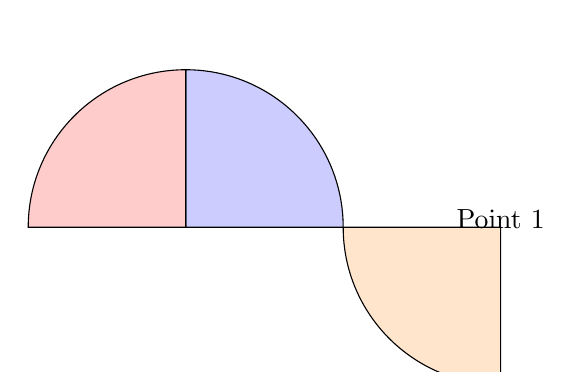
\begin{tikzpicture}

    % starts at 0,0, go to angle 0, radius 2, shape the arc from angle 0 to angle 90 with radius 2
    \draw[fill=blue!20] (0,0) -- (0:2) arc (0:90:2) -- cycle;

    \draw[fill=red!20]  (0,0) -- (90:2) arc (90:180:2) -- cycle;
    \draw[fill=orange!20, shift={(4,0)}]  (0,0) -- (180:2) arc (180:270:2) -- cycle;

    \node at (4,0.1) {Point 1};


\end{tikzpicture}

\subsection{Nodes \& Shapes - Connectons}
   
\begin{tikzpicture}

    % "inner sep" forces real size, if no if text bigger then shapes get bigger to fully wrapp inside text
    \node[draw, 
          shape=circle,
          minimum size=2.1cm,
          inner sep=0pt] (Z) at (0,0) {A};
    \node[draw, 
          shape=rectangle,
          minimum size=2.1cm,
          inner sep=0pt] (Y) at (6,0) {B};

    \draw[->] (Z) -- (Y);

\end{tikzpicture}

Another example:

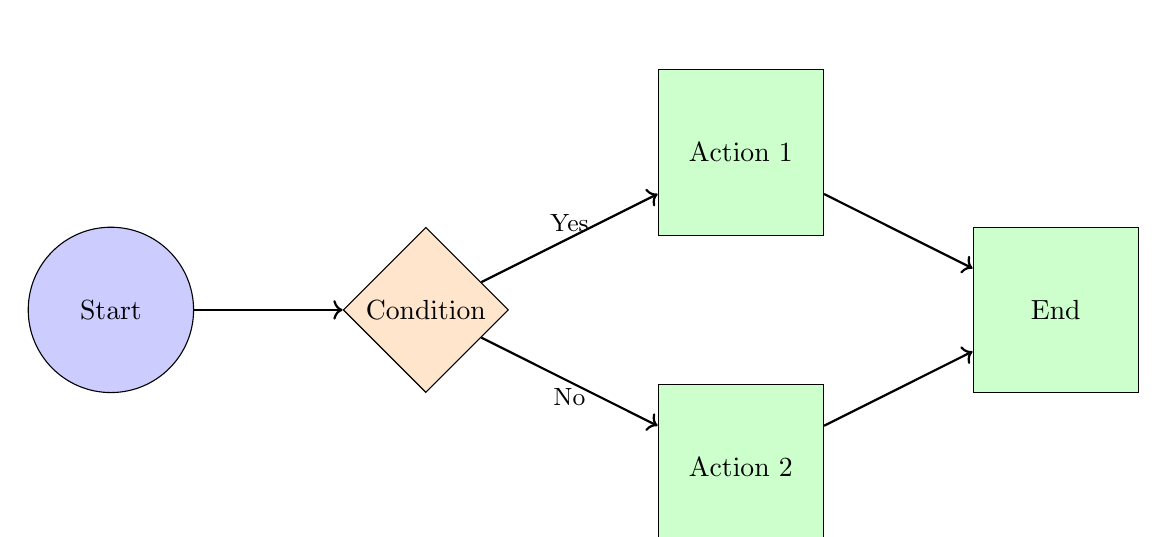
\begin{tikzpicture}[
    % Global style for all nodes
    every node/.style={
        draw,
        minimum size=2.1cm,
        inner sep=0pt,
        align=center
    },
    edgeLabel/.style={
        draw=none,
        fill=none,
        minimum size=0pt,
        inner sep=2pt,
        font=\small
    },
    % Custom styles
    circleNode/.style={circle, fill=blue!20},
    rectNode/.style={rectangle, fill=green!20},
    diamondNode/.style={diamond, aspect=2, fill=orange!20},
    arrow/.style={->, thick}
]

    % Main nodes
    \node[circleNode] (Z) at (0,0) {Start};
    \node[diamondNode] (D) at (4,0) {Condition};
    \node[rectNode] (Y) at (8,2) {Action 1};
    \node[rectNode] (W) at (8,-2) {Action 2};
    
    % Extra node
    \node[rectNode] (End) at (12,0) {End};
    
    % Connections
    \draw[arrow] (Z) -- (D);
    \draw[arrow] (D) -- node[edgeLabel, above]{Yes} (Y);
    \draw[arrow] (D) -- node[edgeLabel, below]{No} (W);
    
    \draw[arrow] (Y) -- (End);
    \draw[arrow] (W) -- (End);

\end{tikzpicture}

\subsection{Transformations}

\begin{tikzpicture}

    \draw[shift={(4,0)}, rotate=45, scale=0.5]
      (0,0) ellipse (3 and 1);
    
    \draw[shift={(12,0)}, rotate=45, scale=0.5]
      (0,0) ellipse (3 and 1);

\end{tikzpicture}

\subsection{3D}

\begin{tikzpicture}
\draw[->] (0,0,0) -- (2,0,0); % x axis
\draw[->] (0,0,0) -- (0,2,0); % y axis
\draw[->] (0,0,0) -- (0,0,2); % z axis
\end{tikzpicture}

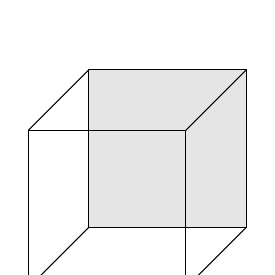
\begin{tikzpicture}

    \fill[gray!20] (0,0,0) -- (2,0,0) -- (2,2,0) -- (0,2,0) -- cycle;
    
    
    \draw (0,0,0) -- (2,0,0) -- (2,2,0) -- (0,2,0) -- cycle;
    \draw (0,0,2) -- (2,0,2) -- (2,2,2) -- (0,2,2) -- cycle;
    
    \draw (0,0,0) -- (0,0,2);
    \draw (2,0,0) -- (2,0,2);
    \draw (2,2,0) -- (2,2,2);
    \draw (0,2,0) -- (0,2,2);

\end{tikzpicture}

\subsubsection{Camera angles}

Here we deonstrate the importance of rotation composition order.

If we srite:

rotate around x
rotate around y
rotate around z

It will be this composition:

rotate\_x(rotate\_y(rotate\_z()))

Rotating a line that is perfectly aligned to axis X around X changes nothing (logic).

So in that is why second and third figures are the same, because in the third figure, rotating around x happens first and does nothing, so still jut y rotation that is the same at what the second figure does.

Also the first figure rotate x last, so even if the rotation angle are the same for y and we just said that rotating around x does nothing in this case (because the line is perfectly parallel tp x), the composition order is y then x, that is why it gave a different result.

\begin{tikzpicture}[rotate around x=45,
                    rotate around y=45,
                    rotate around z=0
                    ]
    \draw (0,0,0) -- (2,0,0);

\end{tikzpicture}

\begin{tikzpicture}[rotate around x=0,
                    rotate around y=45,
                    rotate around z=0
                    ]
    \draw (0,0,0) -- (2,0,0);

\end{tikzpicture}

\begin{tikzpicture}[rotate around y=45,
                    rotate around x=45,
                    rotate around z=0
                    ]
    \draw (0,0,0) -- (2,0,0);

\end{tikzpicture}

\begin{tikzpicture}[rotate around x=0,
                    rotate around y=0,
                    rotate around z=45
                    ]
    \draw (0,0,0) -- (2,0,0);
\end{tikzpicture}


Another example:

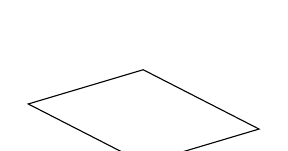
\begin{tikzpicture}[rotate around x=45, rotate around z=30]
\draw (0,0,0) -- (2,0,0) -- (2,2,0) -- (0,2,0) -- cycle;
\end{tikzpicture}
\subsection{Surfaces - PgfPlots}

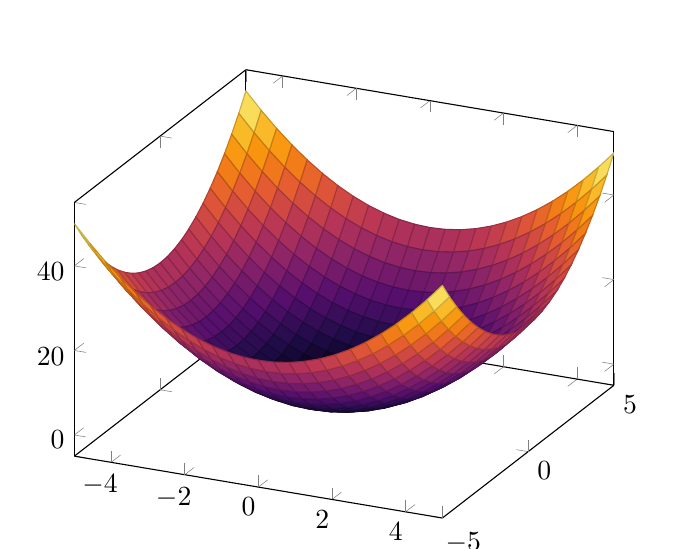
\begin{tikzpicture}
\begin{axis}

    \addplot3[surf] {x^2 + y^2};

\end{axis}
\end{tikzpicture}

\section{For chemists}

\subsection{Simple links}

\chemfig{C-C-O}

\subsection{Links types}

\chemfig{C-C}

\chemfig{C=C}

\chemfig{C~C}

\subsection{Links Angles}

\chemfig{-[:30]C-[:60]=O}
\chemfig{(H-)(H-)C(-H)(-[:55]H)-[:30]C=[:60]O}

\chemfig{C(=[:30]O)
          (=[:270]O)
          (=[:300]
             (H-)
             I
             (-H))
         -C
         }

Isopropanol:

\chemfig{
    CH_3-CH(-[:90]OH)-CH_3
}

\subsection{Rings}

Cyclohexane:

\chemfig{
    *6(------)
}

Benzene:

\chemfig{
    *6(-=-=-=)
}

Another example:

\chemfig{
    *6(-(-CH_3)=-(-OH)-=-)
}

\subsection{Charges}

\chemfig{N^\oplus}

\chemfig{O^\ominus} 

% to not collide with specific chemfig DSL link synthax, group the minus like "{-}"
% so now "-" is just a character, not a special chemfig synthax 
\chemfig{O^{-}} 
\chemfig{O^{+}} 


\end{document}







